%
% This is the LaTeX template file for lecture notes for EE 382V.
%

\documentclass[twoside]{article}
\usepackage{graphicx}
\graphicspath{ {images/} }
\setlength{\oddsidemargin}{0.25 in}
\setlength{\evensidemargin}{-0.25 in}
\setlength{\topmargin}{-0.6 in}
\setlength{\textwidth}{6.5 in}
\setlength{\textheight}{8.5 in}
\setlength{\headsep}{0.75 in}
\setlength{\parindent}{0 in}
\setlength{\parskip}{0.1 in}

%
% The following commands set up the lecnum (lecture number)
% counter and make various numbering schemes work relative
% to the lecture number.
%
\newcounter{lecnum}
\renewcommand{\thepage}{\thelecnum-\arabic{page}}
\renewcommand{\thesection}{\thelecnum.\arabic{section}}
\renewcommand{\theequation}{\thelecnum.\arabic{equation}}
\renewcommand{\thefigure}{\thelecnum.\arabic{figure}}
\renewcommand{\thetable}{\thelecnum.\arabic{table}}

%
% The following macro is used to generate the header.
%
\newcommand{\lecture}[4]{
   \pagestyle{myheadings}
   \thispagestyle{plain}
   \newpage
   \setcounter{lecnum}{#1}
   \setcounter{page}{1}
   \noindent
   \begin{center}
   \framebox{
      \vbox{\vspace{2mm}
    \hbox to 6.28in { {\bf EE 382V: Social Computing
                        \hfill Fall 2018} }
       \vspace{4mm}
       \hbox to 6.28in { {\Large \hfill Lecture #1: #2  \hfill} }
       \vspace{2mm}
       \hbox to 6.28in { {\it Lecturer: #3 \hfill Scribe: #4} }
      \vspace{2mm}}
   }
   \end{center}
   \markboth{Lecture #1: #2}{Lecture #1: #2}
   %{\bf Disclaimer}: {\it These notes have not been subjected to the
   %usual scrutiny reserved for formal publications.  They may be distributed
   %outside this class only with the permission of the Instructor.}
   \vspace*{4mm}
}

%
% Convention for citations is authors' initials followed by the year.
% For example, to cite a paper by Leighton and Maggs you would type
% \cite{LM89}, and to cite a paper by Strassen you would type \cite{S69}.
% (To avoid bibliography problems, for now we redefine the \cite command.)
% Also commands that create a suitable format for the reference list.
\renewcommand{\cite}[1]{[#1]}
\def\beginrefs{\begin{list}%
        {[\arabic{equation}]}{\usecounter{equation}
         \setlength{\leftmargin}{2.0truecm}\setlength{\labelsep}{0.4truecm}%
         \setlength{\labelwidth}{1.6truecm}}}
\def\endrefs{\end{list}}
\def\bibentry#1{\item[\hbox{[#1]}]}

%Use this command for a figure; it puts a figure in wherever you want it.
%usage: \fig{NUMBER}{SPACE-IN-INCHES}{CAPTION}
\newcommand{\fig}[3]{
			\vspace{#2}
			\begin{center}
			Figure \thelecnum.#1:~#3
			\end{center}
	}
% Use these for theorems, lemmas, proofs, etc.
\newtheorem{theorem}{Theorem}[lecnum]
\newtheorem{lemma}[theorem]{Lemma}
\newtheorem{proposition}[theorem]{Proposition}
\newtheorem{claim}[theorem]{Claim}
\newtheorem{corollary}[theorem]{Corollary}
\newtheorem{definition}[theorem]{Definition}
\newenvironment{proof}{{\bf Proof:}}{\hfill\rule{2mm}{2mm}}

% **** IF YOU WANT TO DEFINE ADDITIONAL MACROS FOR YOURSELF, PUT THEM HERE:

\begin{document}
%FILL IN THE RIGHT INFO.
%\lecture{**LECTURE-NUMBER**}{**DATE**}{**LECTURER**}{**SCRIBE**}
\lecture{8 Session 3}{November 10}{Vijay Garg}{Haleigh Walker}

\section{RSA Underlying Mathematics}
\begin{proof}
We want to demonstrate the correctness of our RSA algorithm  and Euler's Theorem for any integer M which is relatively prime to n. \newline
\hspace*{10mm}$M^{\Phi(n)}$ $ \equiv$ $1$ $mod$ $n$ \newline

Here $\Phi(n)$ is the Euler totient function giving numbers of positive integers less than n which are relatively prime to n. For prime numbers p: \newline
\hspace*{10mm}$\Phi(p)$ = p - 1 \newline

Therefore: \newline
\hspace*{10mm}$\Phi(n)$ = $\Phi(p)$ $ \cdot $ $\Phi(q)$ \newline
\hspace*{17mm} = (p - 1) $ \cdot $ (q - 1) \newline
\hspace*{17mm} = n - $ (p + q) $ + 1 \newline

Since d is relatively prime to $\Phi(n)$, its inverse e is in the ring of integers modulo $\Phi(n)$: \newline
\hspace*{10mm}e $ \cdot $ d $ \equiv $ $ 1$ $ mod$ $ \Phi(n)$ \newline

We now want to prove that our equations for encryption and decryption hold true when e and d are chosen correctly. \newline
\hspace*{10mm}D(E(M)) \equiv (E(M))^d \equiv (M^e)^d $ mod $ n = M^{ed} $ mod $ n \newline
\hspace*{10mm}E(D(M)) \equiv (D(M))^e \equiv (M^d)^e $ mod $ n = M^{ed} $ mod $ n \newline
\hspace*{10mm}M^{ed} \equiv $M^{k\Phi(n)+1}$ mod n (for some integer k) \newline

For all M such that p does not divide M \newline
\hspace*{10mm}M^{p - 1} \equiv 1 $ mod $ p \newline
 
We also know that:\newline
\hspace*{10mm} $\Phi(n)$ = $(p - 1) \cdot (q - 1)$ \newline
\hspace*{10mm} $k\Phi(n)$ = $k(p - 1) \cdot (q - 1)$ \newline

Therefore: \newline
\hspace*{10mm}$M^{k\Phi(n)+1}$ = $(M^{p-1})^{k(q-1)} $ \cdot$ $ M$ = $1$ $ \cdot$ $ M$

Since (p - 1) divides $\Phi(n)$, from here we can conclude: \newline
 \hspace*{10mm} $M^{k\Phi(n)+1}$ $\equiv$ $M$ $mod$ $p$ 

Similarly\newline 
\hspace*{10mm}$M^{k\Phi(n)+1}$ \equiv M $ mod $ q

Since $n = pq$, it is therefore implied that for all M \newline
\hspace*{10mm}M^{ed} \equiv $M^{k\Phi(n)+1}$ \equiv M $ mod $ n \newline

Therefore E and D are inverse permutations. 
\end{proof}

\section{Finite Distributive Lattice (FDL)}
The lattice is used to model the search space of the combinatorial optimization problem. We want a parallel algorithm to solve problems with n processes.  
The goal of the combinatorial optimization problem is to find the smallest element in the lattice which satisfies the predicate (feasible solutions). We will assume the bollean predicate B is lattice linear. \newline

Algorithm: getLeastFeasible \newline
 \hspace*{10mm} if predicate is true \newline
 \hspace*{20mm} you are done \newline
 \hspace*{10mm} else \newline
 \hspace*{20mm} there is at least one place you must advance to make the predicate true (at least 1 forbidden) \newline
 
We  will  model the current state of the system with vector G, the global state, where G[i], the state of the process, is maintained at process i.
 
\begin{definition}
Forbidden State: Given a predicate B,  and a vector $G \in L$,  a state G[i] is forbidden if for any vector $H \in L$, where $G \leq H$, if H[i] equals G[i], then B is false for H.\newline

\hspace*{10mm}forbidden(G,i,B) ≡ $\forall H \in L$: $G \leq H$: (G[i] = H[i])\Longrightarrow $$\neg B(H)$.
\end{definition}
 
\begin{definition}
Lattice Linear Predicates: We define a predicate B to be lattice-linear with respect to a lattice L if for any global state G, B is false in G implies that G contains a forbidden state. A boolean predicate B Is lattice-linear with respect to a lattice L iff \newline

\hspace*{10mm}\forall G \in L: \neg $B(G)$ $\Longrightarrow$ \exists $ i $ : forbidden(G, i, B)
\end{definition}
  
\begin{theorem}
$B_1$ is lattice linear $\bigwedge$ $ B_2$ is lattice linear $\Longrightarrow$ $ B_1$ $\bigwedge$ $ B_2$ is lattice linear
\end{theorem}
  
\begin{proof}
Global state G where $B_1$ or $B_2$ is false
(If $B_2$ can never be true, then $ B_1$ $\bigwedge$ $ B_2$ can never be true) \newline
 
We need to show \neg $B(G)$ $ \Longrightarrow$ $\exists i $ : forbidden(G, i, B) \newline
 
Suppose \neg($ B_1$ $\bigwedge$ $ B_2$ ). This  implies  that  one  of the  predicates is  false  and  therefore  from lattice-linearity, a forbidden state exists.
\end{proof} \newline
 
Ex: Smallest possible cut = optimal answer \newline
 
The predicate is true in the blue circles \newline
If the lattice is linear, you can advance to find the optimal solution \newline
We need to make our cut so that we have P1, P2, and P3 true. See Figure 3.1 below. \newline
\begin{center}
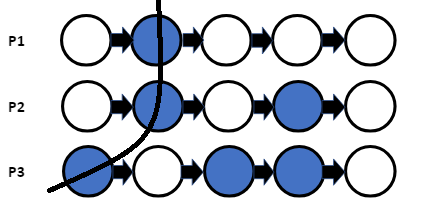
\includegraphics[width=0.4\textwidth]{figure_1_bubbles_with_G.PNG}
\end{center}
\fig{1}{4}{Optimal Solution for Lattice Linear Example}

\subsection{Stable Marriage}
We now illustrate that the lattice-linear predicate detection technique is applicable when the search space is any distributive lattice by applying predicate detection to the stable marriage problem.\newline

The vertices are a set of proposals E that can be made by men to women. We refer to these proposals as events which are executed by n processes {P1, P2 … $P_n$} corresponding to n men. When there are no constraints, we impose a partial order  $\rightarrow p $ on E with n disjoint chains to model the order in which these proposals can be made. Similar to the Gale-Shapely algorithm, each process makes proposals to women in decreasing order of male preferences. In Figure 3.2, black arrows indicate male preference in decreasing order, while red arrows indicate female preferences in increasing order.\newline

\begin{center}
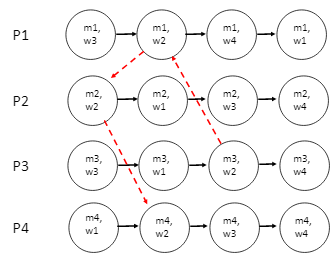
\includegraphics[width=0.4\textwidth]{figure_2_wpref.PNG}
\end{center}
\fig{2}{4}{Male and Female Preferences}
 
w2 preferences in order: m4, m2, m1, m3 \newline

Feasible Predicate: Assignment that gives a stable marriage. \newline

E: set of proposals that can be made by men to women \newline
$ \rightarrow p$: partial order imposed

\begin{definition}
A global state $G \subseteq E$ is consistent if \newline
 \hspace*{10mm}$\forall e$, $f \in  E$ : (e $ \rightarrow p$  f )  $ \bigwedge $  ($f \in  G$) $ \Longrightarrow $ ($e \in G$).
\end{definition}

Looking for male optimal solution that satisfies the feasible solution.

\newline
G = Global State \newline
$B_{stable marriage}$ \equiv B_{sin} (G) \newline
\hspace*{23mm} $\equiv $ frontier of consistent global state G \newline
\hspace*{22mm} $\equiv $ last state in G \newline
\hspace*{22mm} $\equiv $ G satisfies stable marriage predicate iff there is no red arrow pointing from frontier of G to \newline
\hspace*{24mm} any state in G AND G is consistent \newline

Note: Red arrows pointing backwards from G indicate a blocking pair. A red arrow pointing within G also violates matching because it indicates the same woman for two men.

\subsection{Prove Lattice Linear Predicate}
\begin{claim}
Backwards red arrows are forbidden. \newline
\end{claim}

\begin{center}
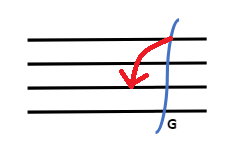
\includegraphics[width=0.4\textwidth]{figure_3_lines_w_G_and_arrow.PNG}
\end{center}
\fig{3}{4}{Backwards Red Arrows}
 
The predicate can only be true if you advance on this process. You must advance at forbidden states to find the optimal solution. \newline
 
This algorithm is more parallel than Gale-Shapely because multiple forbidden states can advance at the same time. \newline

\subsection{Constrained Stable Marriage}
For the constrained stable marriage problem, we have arrows that relate proposals of different processes. In the diagram below, the black arrows indicate the order of proposal. If the process proposes to a circle an arrow is pointing to, it must also propose to the circle from which the arrow originated (See Figures 3.4 and 3.5 below). \newline \newline
\begin{center}
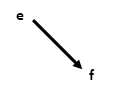
\includegraphics[width=0.2\textwidth]{e_f.PNG}
\end{center}
\fig{4}{4}{If You Include f, You Must Include e}

\begin{center}
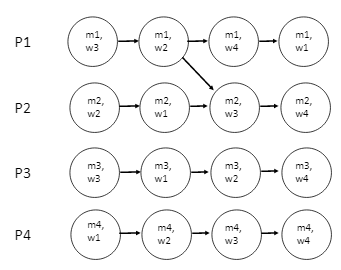
\includegraphics[width=0.4\textwidth]{constrained_stable_marriage.PNG}
\end{center}
\fig{5}{4}{Constrained Stable Marriage}

Backwards black arrows indicate that G is not consistent (future to past). See Figure 3.6 below. \newline

\begin{center}
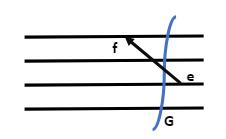
\includegraphics[width=0.4\textwidth]{G_not_consistent.PNG}
\end{center}
\fig{6}{4}{G is not Consistent}

\subsection{Algorithm Applications}
The same algorithm can be applied to multiple problems, such as Market Clearing Price (VCG) and Housing Allocation problems, but the predicate continues to change. \newline
\subsubsection{Market Clearing Price}
For VCG, if you are given a price vector, prices must increase, therefore decreasing prices are forbidden. You can then construct a preferred seller graph (bipartite graph). \newline
Predicate: Market clearing at perfect matching. \newline
We know that without perfect matching, a constricted set exists. \newline
In the minimal set of constricted items, all items are forbidden. \newline
\subsubsection{Housing Allocation}
In the Housing Allocation problem, subset matchings create cycles. Not being part of a cycle is forbidden. 
\end{document}
